\begin{frame}{Scientific context}
	\begin{minipage}{0.75\linewidth}
		\textbf{Context :} Create real-time digital twins of an organ (e.g. liver).
	\end{minipage}
	\begin{minipage}{0.21\linewidth}
		\vspace{-20pt}
		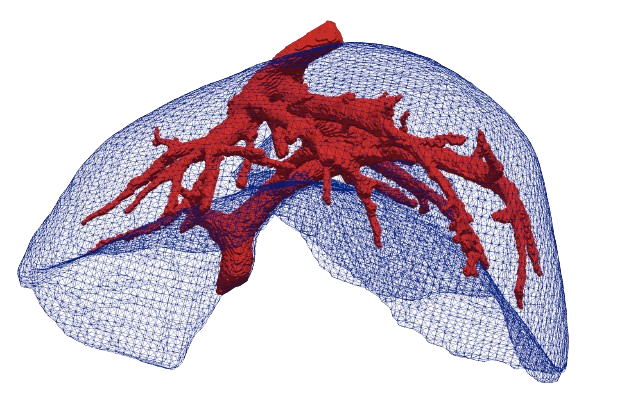
\includegraphics[width=\linewidth]{images/intro/liver.png}
	\end{minipage}
	
	\vspace{5pt}
	\textbf{Objective :} Develop an hybrid \fcolorbox{darkred}{white}{finite element} / \fcolorbox{orange}{white}{neural network} method.
	
	\vspace{1pt}
	\small
	\hspace{130pt} \begin{minipage}{0.14\linewidth}
		\textcolor{darkred}{accurate}
	\end{minipage} \hspace{8pt} \begin{minipage}{0.3\linewidth}
		\textcolor{orange}{quick + parameterized}
	\end{minipage}

	\begin{figure}[!ht]
		\centering
		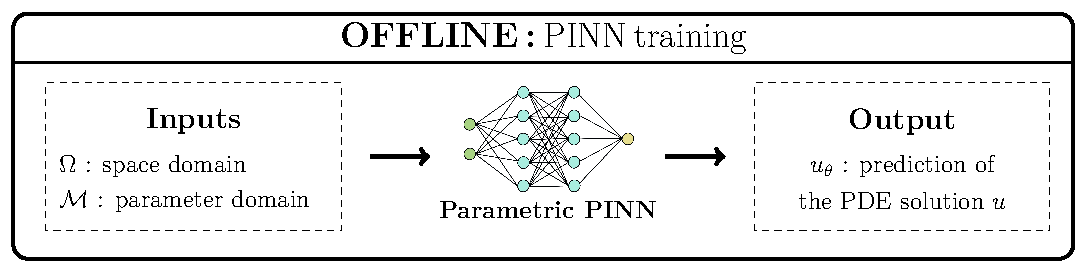
\includegraphics[width=0.7\linewidth]{images/intro/pipeline/offline.pdf}

		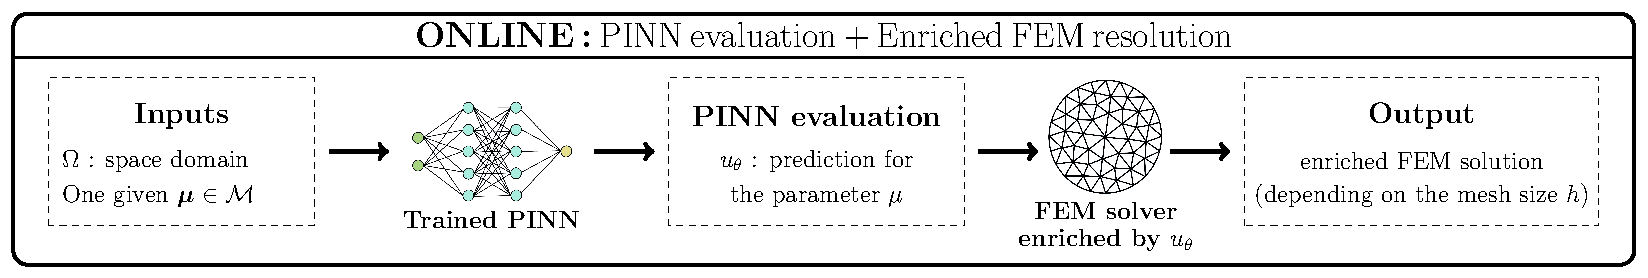
\includegraphics[width=\linewidth]{images/intro/pipeline/online.pdf}
	\end{figure}

	\begin{center}
		\textbf{Complete ONLINE process :} \textcolor{orange}{quick} + \textcolor{darkred}{accurate}
	\end{center}
\end{frame}

\begin{frame}{Heated cavity test case}
	
	
	\only<2>{\textcolor{darkred}{\textbf{Objective:} Simulation on a range of parameters $\bm{\mu} = (\nu,k_f) \in \mathcal{M} = [0.01, 0.1]^2$.}\vspace{5pt}}\only<3>{\textbf{Objective:} Simulation on a range of parameters $\bm{\mu} = (\nu,k_f) \in \mathcal{M} = [0.01, 0.1]^2$.\vspace{5pt}}

	\textbf{Stationary incompressible Navier-Stokes equations (with buoyancy and gravity)\only<1>{\footnote[frame,1]{\textcolor{darkred}{The approach will be shown on this example, but can be extended to other test cases.}}} :}

	We consider \only<1>{$\Omega = [-1,1]^2$ a squared domain}\only<2>{\textcolor{darkred}{$\bm{x}=(x,y)\in\Omega$}}\only<3>{$\bm{x}=(x,y)\in\Omega$} and $\bm{e}_y = (0,1)$.
	
	Find \only<1>{the velocity $\bm{u}=(u_1,u_2)$, the pressure $p$ and the temperature $T$}\only<2>{\textcolor{darkred}{$\bm{U} = (\bm{u},p,T) = (u_1,u_2,p,T)$}}\only<3>{$\bm{U} = (\bm{u},p,T) = (u_1,u_2,p,T)$} such that
	\begin{equation} \label{eq:Pb}
		\left\{\begin{aligned}
			&\only<1>{(\bm{u} \cdot \nabla)\bm{u} + \nabla p - \nu \Delta \bm{u} - g (\beta T + 1)\bm{e}_y}\only<2>{\textcolor{darkred}{R_{mom}(U;\bm{x},\bm{\mu})}}\only<3>{R_{mom}(U;\bm{x},\bm{\mu})} = 0 \;\; \text{in } \Omega \quad &&\text{\small (momentum)} \\
			&\only<1>{\nabla \cdot \bm{u}}\only<2>{\textcolor{darkred}{R_{inc}(U;\bm{x},\bm{\mu})}}\only<3>{R_{inc}(U;\bm{x},\bm{\mu})} = 0 \;\; \text{in } \Omega \quad &&\text{\small (incompressibility)} \\
			&\only<1>{\bm{u} \cdot \nabla T - k_f \Delta T}\only<2>{\textcolor{darkred}{R_{ener}(U;\bm{x},\bm{\mu})}}\only<3>{R_{ener}(U;\bm{x},\bm{\mu})} = 0 \;\; \text{in } \Omega \quad &&\text{\small (energy)} \only<1-2>{\\
			&\text{+ suitable BC}}
		\end{aligned}\right.
		\tag{$\mathcal{P}$}
	\end{equation}
	
	with $g=9.81$ the gravity, $\beta=0.1$ the expansion coefficient, $\nu$ the viscosity and $k_f$ the thermal conductivity. \citep{coulaud_investigations_2024}

	\vspace{5pt}
	

	\only<3>{\textcolor{darkred}{\textbf{Boundary Conditions:}}

	\textbf{No-slip BC :} $\bm{u} = 0$ on $\partial\Omega$ \qquad \textbf{Isothermal BC :} $T = 1$ on the left wall ($x=-1$)\\
	\hspace{180pt}$T = -1$ on the right wall ($x=1$) \\
	\textbf{Adiabatic BC :} $\displaystyle \frac{\partial T}{\partial n} = 0$ on the top and bottom walls ($y=\pm 1$, denoted by $\Gamma_\text{ad}$)
	}
\end{frame}

\begin{frame}{Evaluate quality of solutions}
	In the following, we are interested in three parameters (rising in complexity) :

	\begin{center}
		\textcolor<2>{darkred}{$\bm{\mu}^{(1)} = (0.1,0.1)$}, \textcolor<3>{darkred}{$\bm{\mu}^{(2)} = (0.05,0.05)$} and \textcolor<4>{darkred}{$\bm{\mu}^{(3)} = (0.01,0.01)$}
	\end{center}

	We evaluate the quality of solutions by comparing them to a reference solution.\footnote[frame,1]{Computed on an over-refined mesh ($h=7.10^{-3}$) on a $\mathbb{P}_3^2\times \mathbb{P}_2 \times \mathbb{P}_3$ continuous Lagrange FE space.}

	\vspace{10pt}

	\only<2-4>{\textbf{Reference solution} \; - \; Rayleigh number : \textcolor{darkred}{\only<2>{$Ra = 1\,569.6$}\only<3>{$Ra = 6\,278.4$}\only<4>{$Ra = 156\,960$}}}

	\vspace{3pt}
	\only<2-4>{$\hspace{32pt} u_{1,\text{ref}} \hspace{67pt} u_{2,\text{ref}} \hspace{67pt} p_\text{ref} \hspace{67pt} T_\text{ref}$}
	\vspace{-3pt}

	\begin{center}
		\only<2>{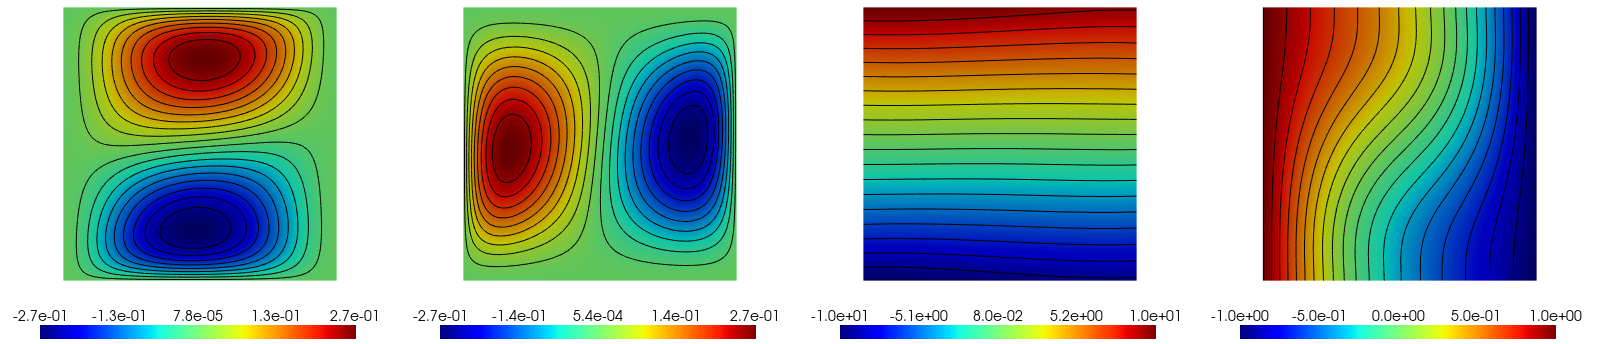
\includegraphics[width=0.98\linewidth]{images/intro/uref/uref1.png}}
		\only<3>{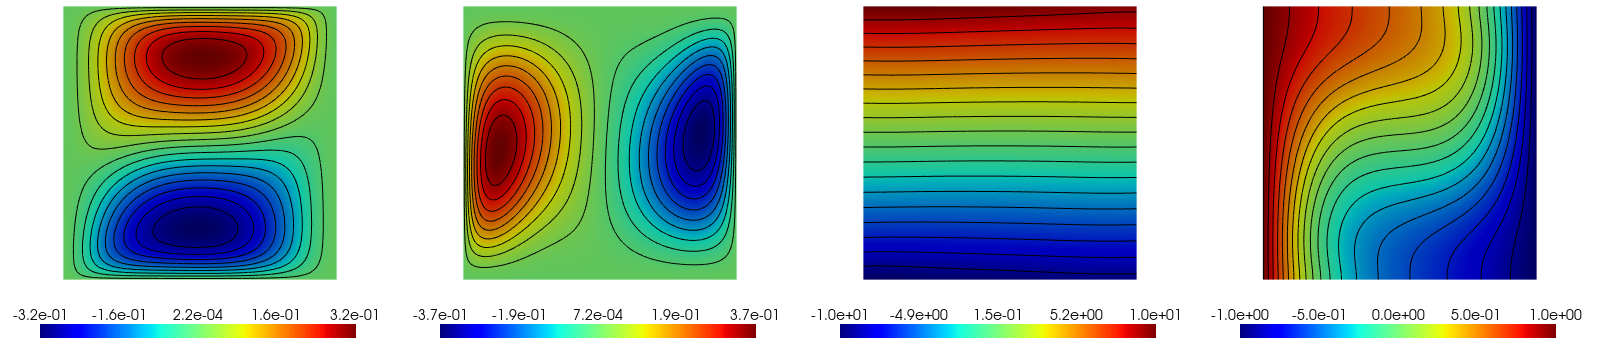
\includegraphics[width=0.98\linewidth]{images/intro/uref/uref2.png}}
		\only<4>{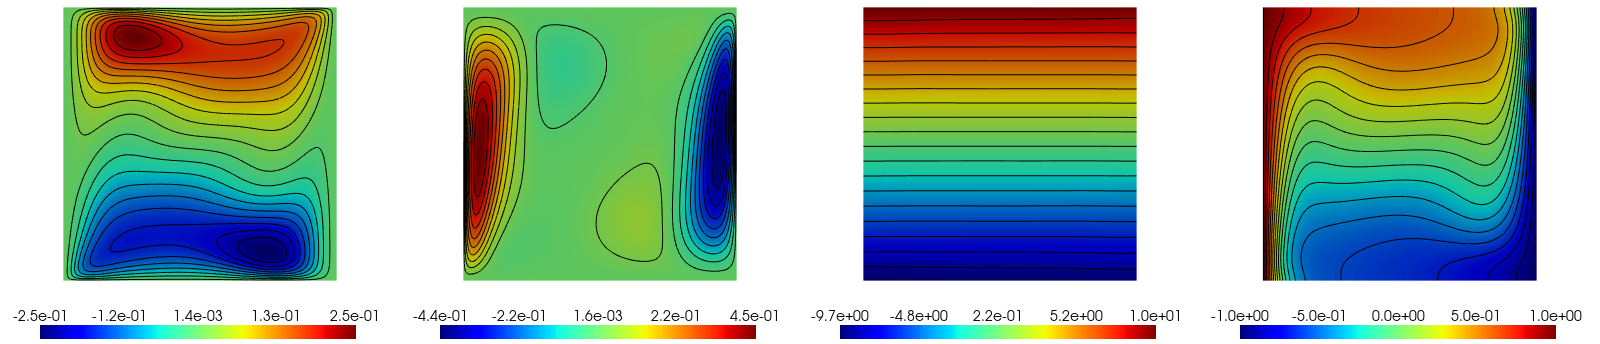
\includegraphics[width=0.98\linewidth]{images/intro/uref/uref3.png}}
	\end{center}

\end{frame}